\chapter{Validation software}

It was important to validate the calculations done in this project continuously. As many of the calculations are not static, but because of inertial forces is was important to visualize these changes as they were happening. It was decided that implementing this feature in GeoMod would be too time consuming because of it's size and complexity. 

It was therefore necessary to create a smaller program that would be able to do the calculations and visualize the results as a form of prototyping. That way, the algorithms could be validated and their practicality determined as fast as possible.


\section{Interface}\label{interfaceSec}

\figref{interface} shows the interface for the completed software created in QtCreator. This section will give a short overview of the functionality of the software, starting with the left menu.

\textsf{Add links} lets the user define a revolute manipulator arm by the \gls{DH} or \textsf{Add default links} can be used to insert a predefined manipulator. By selecting a specific link in the list, it's variables can be viewed and changed in the \textsf{Weight} and \textsf{Joint angle} section. A start and end angle can be defined for each link with the \textsf{Set start/end} button. By pressing the \textsf{to start/end} button the whole manipulator will animate between these configurations over a time specified as in \textsf{Animation time}. The \textsf{Print robot} button will print the homogeneous transformation matrix for each link and the robot as a whole to the console. \textsf{Include dynamic effects} can be toggled off to exclude those contributions from the calculations.

\begin{figure}[h!]
    \centering
    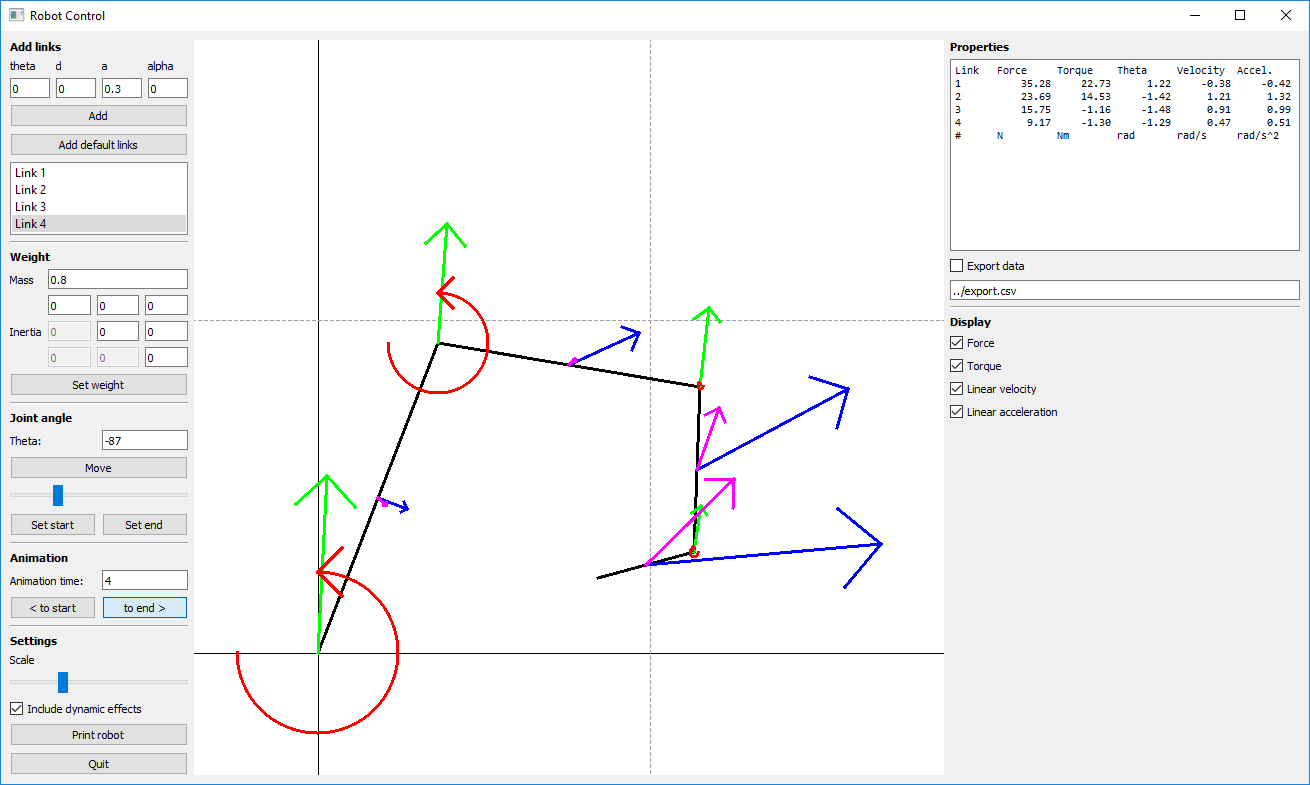
\includegraphics[width=\textwidth]{robot_control_interface5}
    \caption{Main interface of \textit{Robot Control} validation software}
    \label{interface}
\end{figure}

The central area shows the robot together with some relevant vectors for each link. Force and torque in green and red respectively while blue and magenta for the linear velocity and acceleration. The length of the arrows displays a normalized magnitude of that vector. Graphics can be panned and zoomed with the middle mouse button.

Lastly, the right hand side shows useful information for each link and are updated continuously. These are helpful properties used for debugging and validation. If \textsf{Export data} is checked these variables will be saved to a csv-file for each step in the animation. Under \textsf{Display} each of the graphical arrows can be turned on and off

\section{Class overview}

This section will give a short overview of the two most important classes for the dynamic calculations. Listing 5.1 shows the \texttt{Link} class. This class stores all properties needed to define a link and it's current state. When a change is made to the joint angle \texttt{q} the value and the time it were calculated is stored, (line 7 and 8). The angular joint velocity is then calculated in \texttt{newton\_euler\_forward()} with \eqref{omega_calc}, similar for the joint acceleration. \Crefrange{d_der}{d_derder} has been used to find the velocity and acceleration of the link with respect to the inertial reference frame. The force and torque is calculated as part of the \texttt{newton\_euler\_backward()} method.

\lstinputlisting[caption={\texttt{Link.h}, simplified version}]{./snippet/Link.h}\label{Link}

\begin{equation}\label{omega_calc}
\dot{q} = \frac{\Delta q}{\Delta t}=\frac{q-q\_prev}{clock()-last\_update}
\end{equation}

\lstinputlisting[caption={\texttt{Robot.h}, simplified version}]{./snippet/Robot.h}\label{Robot}

The \texttt{Robot} class can be seen in Listing 5.2. Links that make up the robot are stored in a c++ vector (line 4). Many of the calculations is done by looping through this vector. The function \texttt{newtonEuler()} is one of them and perform the dynamic calculations as described in \algref{nefAlgo}.

In addition, multiple mathematical classes like matrices and vectors that handle algebraic operations were created.

\section{Animation}

As mentioned in section \ref{interfaceSec} a start and end angle, $\theta_0$ and $\theta_1$ is stored for each link. By evaluating the desired animation length and elapsed time an animation percentage $\tau$ is calculated. This value is passed to the method \texttt{Robot::animate(percentage)} which calculates the joint angle for each joint by \eqref{quintic}. This is a 5th degree polynomial used for trajectory planning with velocity and acceleration equal to zero at the start and end of the trajectory. See \figref{plot_position}.

\begin{equation}\label{quintic}
\theta\left ( \tau \right ) = \theta_0 + \left ( \theta_1 - \theta_0\right )\left ( 6 \tau^5-15\tau^4 + 10\tau^3\right )
\end{equation}

When using the software, the \textsf{default links} come predefined with start and end angles as in \figref{animation}. This is a clockwise rotation for link one and anticlockwise for link two and three.

\begin{figure}[ht!]
\begin{subfigure}[b]{0.32\textwidth}
    \centering
    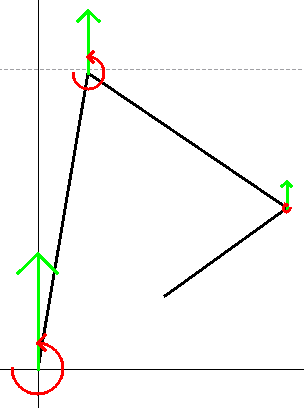
\includegraphics[width=\linewidth]{pos_start}
    \caption{Animation start}
\end{subfigure}
\hfill
\begin{subfigure}[b]{0.4\textwidth}
    \centering
    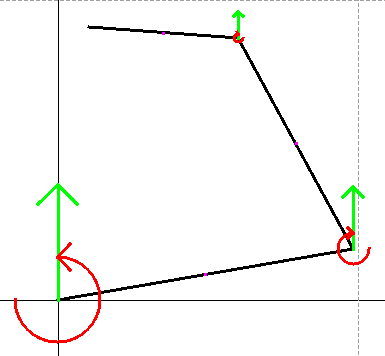
\includegraphics[width=\linewidth]{pos_end}
    \caption{Animation end}
\end{subfigure}
\caption{Start and end of animation for default links.}
\label{animation}
\end{figure}
